\documentclass[8pt, a4paper]{article}
\usepackage{multicol}
\usepackage{listings}
\usepackage{geometry}
\usepackage{graphicx}
\usepackage{caption}
\usepackage{xstring}

\geometry{margin=0.5cm}
\graphicspath{{img}}

\pagenumbering{gobble}
\date{}

\lstdefinestyle{customstyle}{
    basicstyle=\ttfamily\scriptsize,
    breakatwhitespace=true,         
    breaklines=true,                 
    captionpos=t,                    
    keepspaces=false,                 
    showspaces=false,                
    showstringspaces=false,
    showtabs=false,                  
    frame=single,
    tabsize=1
}

\renewcommand\lstlistingname{}
\DeclareCaptionFormat{listing}{}
\captionsetup[lstlisting]{labelformat=empty}

\newcommand{\lstinputwithcaption}[2]{%
  \lstinputlisting[caption={\texttt{#2}}]{#1}%
}
\newcommand{\codeListing}[6] {

  \begin{multicols}{2}
    \lstinputwithcaption{#1}{#2}

    \columnbreak

    \lstinputwithcaption{#3}{#4}

  \end{multicols}

  \begin{center}
    \includegraphics[scale=#5]{#6}
  \end{center}

}

\lstset{style=customstyle}

\begin{document}

NAMA: Radinal Shidiq Saragih

KELAS: IF C 2023

NPM: 5520123104

\begin{enumerate}
  \item Buatlah program untuk mengilustrasikan operator increment

    \begin{multicols}{2}

      \lstinputwithcaption{./code/src/operator\_increment/Main.java}{Main.java}

      \columnbreak

      \begin{center}
        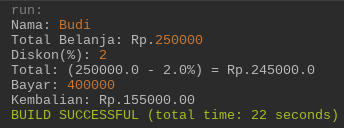
\includegraphics[scale=0.6]{OUTPUT1.png}
      \end{center}

    \end{multicols}

  \item Buatlah program untuk menghitung luas persegi panjang dengan nilai 
    panjang = 50 dan lebar = 45 dengan nama class PersegiPanjang

    \codeListing
      {./code/src/luas\_persegi/PersegiPanjang.java}{PersegiPanjang.java}
      {./code/src/luas\_persegi/Main.java}{Main.java}
      {0.6}{OUTPUT2.png}


  \item Buatlah program untuk menghitung persamaan kuadrat dengan 
    rumus $ b^2 - 4ac $ dengan nilai a=2, b=10, c=5 dengan nama class 
    PersamaanKuadrat

    \codeListing
      {./code/src/persamaan\_kuadrat/PersamaanKuadrat.java}{PersamaanKuadrat.java}
      {./code/src/persamaan\_kuadrat/Main.java}{Main.java}
      {0.6}{OUTPUT3.png}

  \item Buatlah program untuk menghitung proses penjumlahan, pengurangan, perkalian,
    dan pembagian dengan dua bilangan x = 22 dan y == 33 dengan nama class  OperasiMatematika

    \codeListing
      {./code/src/operasi\_matematika/OperasiMatematika.java}{OperasiMatematika.java}
      {./code/src/operasi\_matematika/Main.java}{Main.java}
      {0.6}{OUTPUT4.png}

  \item Buatlah program untuk menghitung luas segitiga dengan a = 6 dan b = 8
    dengan nama class Segitiga. 
  \item Buatkan juga program untuk mencari nilai c
    menggunakan rumus pythagoras setelah itu hitunglah keliling dari segitiga tersebut.

    \codeListing
      {./code/src/segitiga/Segitiga.java}{Segitiga.java}
      {./code/src/segitiga/Main.java}{Main.java}
      {0.6}{OUTPUT5.png}

\end{enumerate}

\end{document}
